\documentclass[12pt]{report}

\usepackage{setspace}
\renewcommand{\baselinestretch}{1.5}
\usepackage{float}
\usepackage{lipsum}
\usepackage{graphicx}
\usepackage{subcaption}
\usepackage[table,xcdraw,dvipsnames]{xcolor}
\usepackage{titlesec}
\usepackage{titletoc}
\usepackage{titling}
\usepackage[T1]{fontenc}
\usepackage[utf8x]{inputenc}
\usepackage{amsmath}
\usepackage{caption}
\usepackage{adjustbox}
%\usepackage[a4paper,margin=0.5in]{geometry}
\usepackage[a4paper,%
            left=2cm,right=2cm,top=1cm,bottom=2cm,%
            footskip=-1cm]{geometry}
\usepackage[normalem]{ulem}
\usepackage[none]{hyphenat}
\usepackage[hidelinks]{hyperref}
\PassOptionsToPackage{hyphens}{url}\usepackage{hyperref}
\useunder{\uline}{\ul}{}

% No hyphenation (word wrapping) with text justification
\tolerance=1
\emergencystretch=\maxdimen
\hyphenpenalty=10000
\hbadness=10000

% Replace table caption name
\usepackage{caption}
\captionsetup[table]{name=Tableau}

% For toc, lot and lof
\usepackage[titles]{tocloft}

% For liste of figures and tables!
\graphicspath{{./images/}}
\usepackage{array}

% Disable auto indentation globally
\setlength{\parindent}{0pt}

% Font options
\usepackage{mathptmx}
%\usepackage{tgtermes}
%\usepackage{tgpagella}
%\usepackage{helvet}
%\usepackage{tgbonum}

% fancy logo for page numbers!
\usepackage{fancyhdr,blindtext,tikz}
\usepackage{lastpage,refcount}



% Box frame for figures #\fbox{}
\setlength{\fboxsep}{0pt}
\setlength{\fboxrule}{0.69pt}

% Options: Sonny, Lenny, Glenn, Conny, Rejne, Bjarne, Bjornstrup
\usepackage[Conny]{fncychap}

%package for inserting raw text files
\usepackage{verbatim}
\usepackage{listings}

% Redifining from 0.1 to 1 ... 2 ... and so on
\renewcommand{\thesection}{\arabic{section}}

% Renaming Bibliography name
\renewcommand\bibname{Bibliographie}

% Bibliography styling
\bibliographystyle{plain}

% Redifining from 1.1 to 1.a ... 1.b ... and so on
%\renewcommand{\thesubsection}{\alph{subsection}}

% Part rules
\titlecontents{part}[1em]
{\vskip 0.5ex}%
{}% numbered sections formatting
{\itshape\scshape}% unnumbered sections formatting
{}%

% Chapter rules
\titlecontents{chapter}[1em]
{\vskip 0.5ex}%
{}% numbered sections formatting
{\itshape\scshape}% unnumbered sections formatting
{\titlerule*[0.3pc]{.}\contentspage}%

% Section rules
\titlecontents{section}[1em]
{\vskip 0.2ex}%
{\hspace{0.15in}\contentslabel{0.13in}.\hspace{0.1in}}% numbered sections formatting
{\itshape}% unnumbered sections formatting
{\titlerule*[0.3pc]{.}\contentspage}%

% Subsection rules
\titlecontents{subsection}[3.5em]
{}%
{\contentslabel{0.10in}\hspace{0.25in}}% numbered sections formatting
{}% unnumbered sections formatting
{\titlerule*[0.3pc]{.}\contentspage}%

% Custom colors!
\definecolor{MYCOL}{HTML}{00318A}

% List of Figures settings:
\renewcommand{\listfigurename}{Liste Des Figures}
\renewcommand{\cftloftitlefont}{\vspace*{-0.6in}\hfill\color{Black}\fontsize{35}{43}\bfseries}
\renewcommand{\cftafterloftitle}{\hfill}
\setlength{\cftfigindent}{0pt} % left aligned Fig entries
\renewcommand{\cftfigpresnum}{Figure } % put before the number
\renewcommand{\cftfigaftersnum}{:} % put before the number
\addtolength{\cftfignumwidth}{2.5em} % extra space for \cftpresnum

% List of Tables settings:
\renewcommand{\listtablename}{Liste Des Tableaux}
\renewcommand{\cftlottitlefont}{\vspace*{-0.6in}\hfill\color{Black}\fontsize{35}{43}\bfseries}
\renewcommand{\cftafterlottitle}{\hfill}
\setlength{\cfttabindent}{0pt} % left aligned Tab entries
\renewcommand{\cfttabpresnum}{Tableau } % put before the number
\renewcommand{\cfttabaftersnum}{:} % put before the number
\addtolength{\cfttabnumwidth}{2.5em} % extra space for \cftpresnum

% Table of contents settings:
\renewcommand{\contentsname}{Table Des Matières}

\usepackage[framemethod=TikZ]{mdframed}

% For the box (theme)
\mdfdefinestyle{MyFrame}{%
    linecolor=black,
    outerlinewidth=2pt,
    roundcorner=0pt,
    innertopmargin=13pt,
    innerbottommargin=13pt,
    innerrightmargin=20pt,
    innerleftmargin=20pt,
    backgroundcolor=gray!10!white}


% My custom page style
\fancypagestyle{myfancy}{%   
   \fancyhf{}%
   \fancyfoot[C]{\tikz[baseline={(0,0)},anchor=center] \node[label={center:\thepage}]{\includegraphics[scale=.037]{../images/cloud.png}};}%
   \renewcommand{\headrulewidth}{0pt}%
   \renewcommand{\footrulewidth}{0pt}%
   \fancyhead{}
   \fancyfoot{}
   \fancyfoot[C]{\vspace{-0.35in}\textcolor{Gray}{\Large{Page}}\hspace{0.04in} \large{\thepage}\hspace{0.07in}\large{|}\hspace{0.07in}\large{\pageref{LastPage}}}
}%
\pagestyle{empty}

% Custom environment
\newenvironment{changemargin}[2]{%
\begin{list}{}{%
\setlength{\topsep}{0pt}%
\setlength{\leftmargin}{#1}%
\setlength{\rightmargin}{#2}%
\setlength{\listparindent}{\parindent}%
\setlength{\itemindent}{\parindent}%
\setlength{\parsep}{\parskip}%
}%
\item[]}{\end{list}}

% 'myfancy' page styling is also applied on chapters!
\usepackage{etoolbox}
\patchcmd{\chapter}{\thispagestyle{empty}}{\thispagestyle{myfancy}}{}{}

\titleformat{\chapter}
{\centering\fontsize{40}{50}\bfseries\color{Black}\scshape}
{}
{}
{\vspace{-1.7in}{\color{Black} \rule{\linewidth}{1.2mm} }}[\vspace{-0.35in}{\color{Black} \rule{\linewidth}{1.2mm} }\vspace{-1in}]

\titleformat{\section}
{\Large\bfseries\color{Black}}
{\thesection.\hspace{0.08in}}
{0em}
{}[\titlerule]

\titleformat{\subsection}
{\large\bfseries\color{Black}}
{\hspace{0.25in}\thesubsection\hspace{0.08in}}
{0em}
{}[]

\titleformat{\subsubsection}
{\bfseries\large}
{\hspace{0.40in}}
{0em}
{}[]

\newenvironment{myindentpar}[1]%
  {\begin{list}{}%
          {\setlength{\leftmargin}{#1}}%
          \item[]%
  }
  {\end{list}}

\usepackage{tikz}
\usetikzlibrary{calc}

\usepackage{fullwidth}




\begin{document}

\begin{titlepage}

   \begin{tikzpicture}[remember picture, overlay]
      \draw[line width = 2pt] ($(current page.north west) + (0.25in,-0.25in)$) rectangle ($(current page.south east) + (-0.25in,0.25in)$);
   \end{tikzpicture}

   \begin{center}
       \vspace*{-0.4in}

       \begin{large}

           République Algérienne Démocratique et Populaire

           Ministère de l'Enseignement Supérieur et de la Recherche Scientifique

           Université M'Hamed Bougara de Boumerdès

       \end{large}

       \vspace{0.1in}

    \begin{figure}[h]
    \centering
        
\includegraphics[width = 1.5in, height = 1in]{../images/UnivUMBB.jpg}
    \end{figure}
     \vspace*{-0.1in}
    \large{Faculté des Sciences}
    \\
    \vspace*{-0.1in}
    \large{Département d'informatique}
   \end{center}

    \hspace{0.2in}
    \large{\textbf{Domaine \,\; :}  Mathématiques Informatique}
    \kern 1in
    \large{\textbf{Année universitaire :}}

    \hspace{0.2in}
    \large{\textbf{Filière \quad\,\,\, :}  Informatique}
    \kern 2.65in
    2021 / 2022

    \hspace{0.2in}
    \large{\textbf{Spécialité \, :}  Technologie de l'information}

    \begin{center}
        \begin{large}

            \vspace{0.1in}

            \textit{\textbf{\uline{Projet fin d'étude}}}
        
        \end{large}

        \vspace{0.3in}

        \textit{\Huge{\textbf{\uline{Thème}}}}

        \vspace{0.2in}

        \begin{mdframed}[style=MyFrame]
            \begin{center}
            \color{Black}
              \Large{\textbf{La segmentation et Comptage des cellules biologiques}}

              \Large{\textbf{dans images de microscope par apprentissage profond}}
            \end{center}
        \end{mdframed}
    \end{center}

    \vspace{0.4in}

    \hspace{0.2in}
    \textit{\textbf{Présenté par :}}

    \hspace{0.2in}
    Gharbi Aghiles

    \hspace{0.2in}
    Neggazi Mohamed Lamine

\end{titlepage}

\newpage

\vspace*{0.2in}

\thispagestyle{empty}

\begin{center}
    {\color{Black} \rule{3in}{1.4mm} }\\
    \vspace{0.1in}
    \scshape{\fontsize{34}{46}{\bfseries{\color{Black}{Résumé}}}}
    \\
    \vspace{0.6in}
\end{center}
\cftaddtitleline{toc}{part}{\vspace{-0.12in}\color{Black}{Résumé}}{}
\begin{changemargin}{0.9cm}{0.9cm}
\hspace*{0.16in}
\end{changemargin}

Le comptage de cellules est une tâche fastidieuse qui bénéficierait grandement de l'automatisation. Le comptage précis des cellules fournit des informations quantitatives essentielles et joue un rôle clé dans la recherche biologique ainsi que dans les applications industrielles et biomédicales. Malheureusement, la méthode de comptage manuel couramment utilisée demande beaucoup de temps, mal standardisée et n'est pas reproductible. La tâche est rendue encore plus difficile par le chevauchement des cellules. la mauvaise qualité de l'imagerie ... , nous décrivons ici un réseau de neurones convolutionnel qui vas segmenter les cellules comme une première phase, et les compter dans la seconde phase.

\vspace{1in}

\begin{changemargin}{0.9cm}{0.9cm}
Mots clés : CNN, Comptage des cellules, segmentation d'image
\end{changemargin}

\newpage

\vspace*{0.2in}

\thispagestyle{empty}

\begin{center}
    {\color{Black} \rule{3in}{1.4mm} }\\
    \vspace{0.1in}
    \scshape{\fontsize{34}{46}{\bfseries{\color{Black}{Abstract}}}}
    \\
    \vspace{0.6in}
\end{center}
\cftaddtitleline{toc}{part}{\vspace{-0.12in}\color{Black}{Abstract}}{}
\begin{changemargin}{0.9cm}{0.9cm}
\hspace*{0.16in}

Cell counting is a tedious task that would benefit greatly from automation. Accurate cell counting provides essential quantitative information and plays a key role in biological research as well as industrial and biomedical applications. Unfortunately, the commonly used manual counting method is time consuming, poorly standardized and not reproducible. The task is made even more difficult by overlapping cells and poor imaging quality. In this paper we describe a convolutional neural network that will segment the cells as a first phase, and count them in the second phase.

\end{changemargin}

\vspace{1in}

\begin{changemargin}{0.9cm}{0.9cm}
Keywords: CNN, cell segmentation, cell counting, convolutional neural networks
\end{changemargin}

\newpage

\cftaddtitleline{toc}{part}{\vspace{-0.12in}\color{Black}{Table des matières}}{}
\tableofcontents

\newpage

\cftaddtitleline{toc}{part}{\vspace{-0.12in}\color{Black}{Liste des figures}}{}
\listoffigures

\newpage

\cftaddtitleline{toc}{part}{\vspace{-0.12in}\color{Black}{Liste des tableaux}}{}
\listoftables

\addtocontents{toc}{\protect\renewcommand{\protect\cftsecleader}{\protect\cftdotfill{\protect\cftsecdotsep}}}

\addtocontents{lof}{\protect\thispagestyle{empty}}
\addtocontents{lot}{\protect\thispagestyle{empty}}
\addtocontents{toc}{\protect\thispagestyle{empty}}

\newpage

\pagestyle{myfancy}

\vspace*{-0.2in}

\setcounter{page}{1}

\begin{center}
    {\color{Black} \rule{6.2in}{1.4mm} }\\
    \vspace{0.1in}
    \scshape{\fontsize{34}{46}{\bfseries{\color{Black}{General Introduction}}}}
    \\
    \vspace{0.5in}
\end{center}
\addcontentsline{toc}{chapter}{\vspace{-0.12in}\color{Black}{General Introduction}}
\hspace*{0.16in}

Blood carries out many vital functions as it circulates through the body. It transports oxygen from the lungs to other body tissues and carries away carbon dioxide. It carries nutrients from the digestive system to the cells of the body, and carries away wastes for excretion by the kidneys. Blood helps our body fight off infectious agents and inactivates toxins, stops bleeding through its clotting ability, and regulates our body temperature. Doctors rely on many blood tests to diagnose and monitor diseases. Some tests measure the components of blood itself; others examine substances found in the blood to identify abnormal functioning of various organs. Hence, we here propose a software system which will assist pathologists to detect blood cell count and help to find out the diseases. This information can be very helpful to a physician who, for example, is trying to identify the cause of a patient's diseases.

Earlier hematologists were performing microscopic Copied selected text to selection primary: examination and counting of blood cells manually, which  was very time-consuming and tedious process. Also, the accuracy of counting mainly depends on their expertise skill and their physical conditions, and because of cells complex nature, it still remains a challenging task to segment cells from its background and count them automatically.\\
<--- --->\\

This thesis is presented in four chapters:\\

\textbf{Chapter 1 State of the art:}\\
\textbf{Chapter 2 Elaboration, Conception of multiple architecture and comparative study:}\\
\textbf{Chapter 3 Dataset collection:}\\
\textbf{Chapter 4 Implementation and experiments:}\\

\newpage

\vspace*{\fill}
\begin{center}
    {\color{Black} \rule{\linewidth}{1.2mm} }\\
\vspace{0.25in}
 {\centering\fontsize{30}{40}{\bfseries{\color{Black}{\scshape{Chapitre 0 : Blood cell}}}}}
\vspace{0.35in}\\
    {\color{Black} \rule{\linewidth}{1.2mm} }
\end{center}
\vspace*{\fill}
\addcontentsline{toc}{chapter}{\color{Black}{Chapitre 0 : Blood cell}}
\setcounter{section}{0}

\newpage

\section{Definition}
\vspace{0.2in}
\hspace*{0.16in}

A blood cell, also called a hematopoietic cell, hemocyte, or hematocyte, is a cell produced through hematopoiesis and found mainly in the blood. Major types of blood cells include red blood cells (erythrocytes), white blood cells (leukocytes), and platelets (thrombocytes). Together, these three kinds of blood cells add up to a total 45\% of the blood tissue by volume, with the remaining 55\% of the volume composed of plasma, the liquid component of blood. \textsuperscript{\cite{hopkins1993human}}\\

\vspace{0.1in}

\begin{figure}[h]
\centering
  \vspace{-0.1in}
    \centerline{\fbox{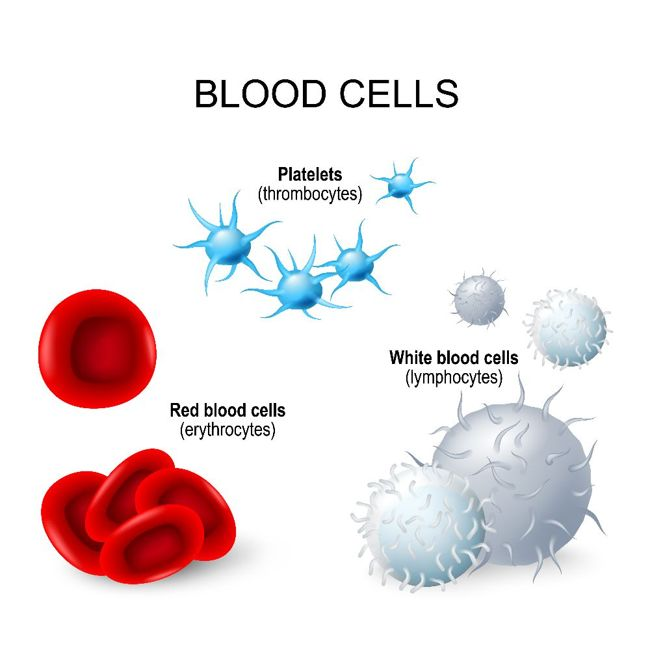
\includegraphics[width = 4in, height = 3.1in]{../images/BloodCells.jpg}}}
    \caption{Blood cells}
\end{figure}

That said, there are three main types of blood cells:

\subsection{Red Blood Cells}

Red blood cells (RBCs) are the cells which carry fresh oxygen all over the human body. This is important to our health. They are round with a flattish, indented center, like doughnuts without a hole. 
The hemoglobin is the protein found inside the red blood cell, and it's main purpose is carrying oxygen.

Most people don't think about their red blood cells unless they have a disease that affects these cells. Problems with red blood cells can be caused by illnesses or a lack of iron or vitamins. Some diseases of the red blood cells are inherited.

Diseases of the red blood cells include many types of anemia. This is a condition in which there are too few red blood cells to carry enough oxygen all over the body.

\newpage

People with anemia may have red blood cells that have an abnormal shape or that look normal, larger than normal, or smaller than normal.

Symptoms of anemia include tiredness, fast heart rate, pale skin, feeling cold, and, in severe cases, heart failure. Children who don't have enough healthy red blood cells grow and develop more slowly than other children. These symptoms show how important red blood cells are to your daily life. \textsuperscript{\cite{Department_2022_rochester}}

\subsection{White Blood Cells}

On the other hand, White Blood Cells (WBCs), also known as leukocytes, are the ones responsible for protecting the human body from infections. As part of the immune system, These cells circulate in the blood and respond to injury or illness. They travel through the bloodstream searching for infections. Then, they notify other WBCs of their location to help defending against attacks from other unknown organisms. Once the army of WBCs arrive, they fight the invader by producing antibody proteins to attach to the organism and destroy it. \textsuperscript{\cite{Attacking_Any_Unknown_2022_clevelandclinic}}

White Blood Cells are divided into five types:

\begin{itemize}
  \item \textbf{Neutrophils:} Help protect your body from infections by killing bacteria, fungi and foreign debris.
  \item \textbf{Lymphocytes:} Consist of T cells, natural killer cells and B cells to protect against viral infections and produce proteins to help you fight infection (antibodies).
  \item \textbf{Eosinophils:} Identify and destroy parasites, cancer cells and assists basophils with your allergic response.
  \item \textbf{Basophils:} Produces an allergic response like coughing, sneezing or a runny nose.
  \item \textbf{Monocytes:} Defend against infection by cleaning up damaged cells.
\end{itemize}

\vspace{0.1in}

\begin{figure}[H]
\centering
  \vspace{-0.1in}
    \centerline{\fbox{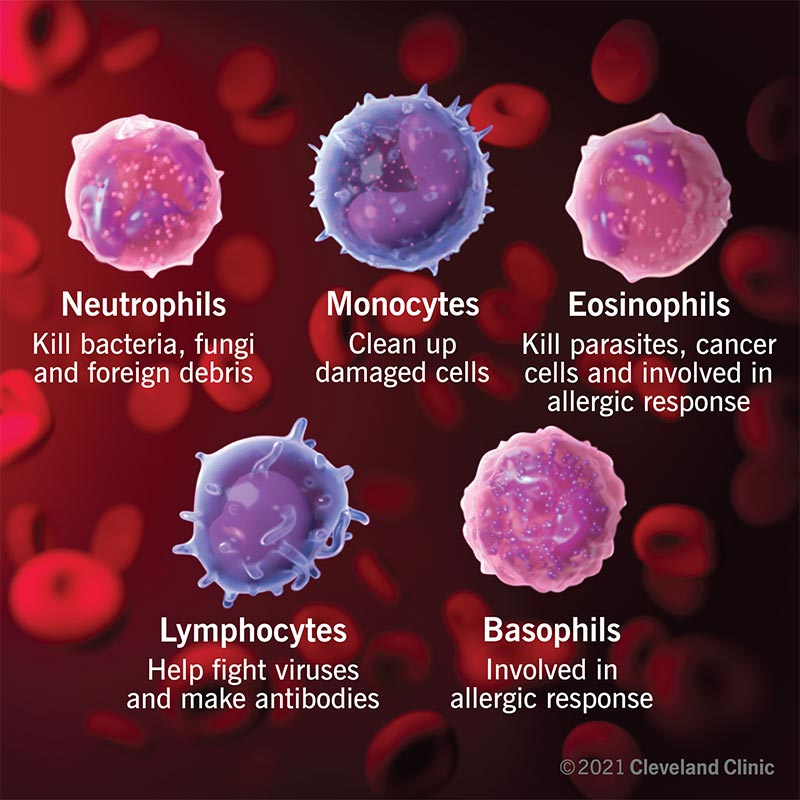
\includegraphics[width = 3.1in, height = 2.5in]{../images/white_blood_cells.jpg}}}
    \caption{The five types of White Blood Cells}
\end{figure}

\subsection{Platelets}

Platelets help prevent blood loss at sites of vascular injury. To do this, they adhere, aggregate and form a procoagulant surface favorizing thrombin generation and fibrin formation. In addition, platelets express and release substances that promote tissue repair and influence processes such as angiogenesis, inflammation and the immune response. They contain large secretable pools of biologically active proteins, while newly synthesized active metabolites are also released. \textsuperscript{\cite{nurden2008platelets}}

\vspace{0.2in}

\begin{figure}[h]
\centering
  \vspace{-0.1in}
    \centerline{\fbox{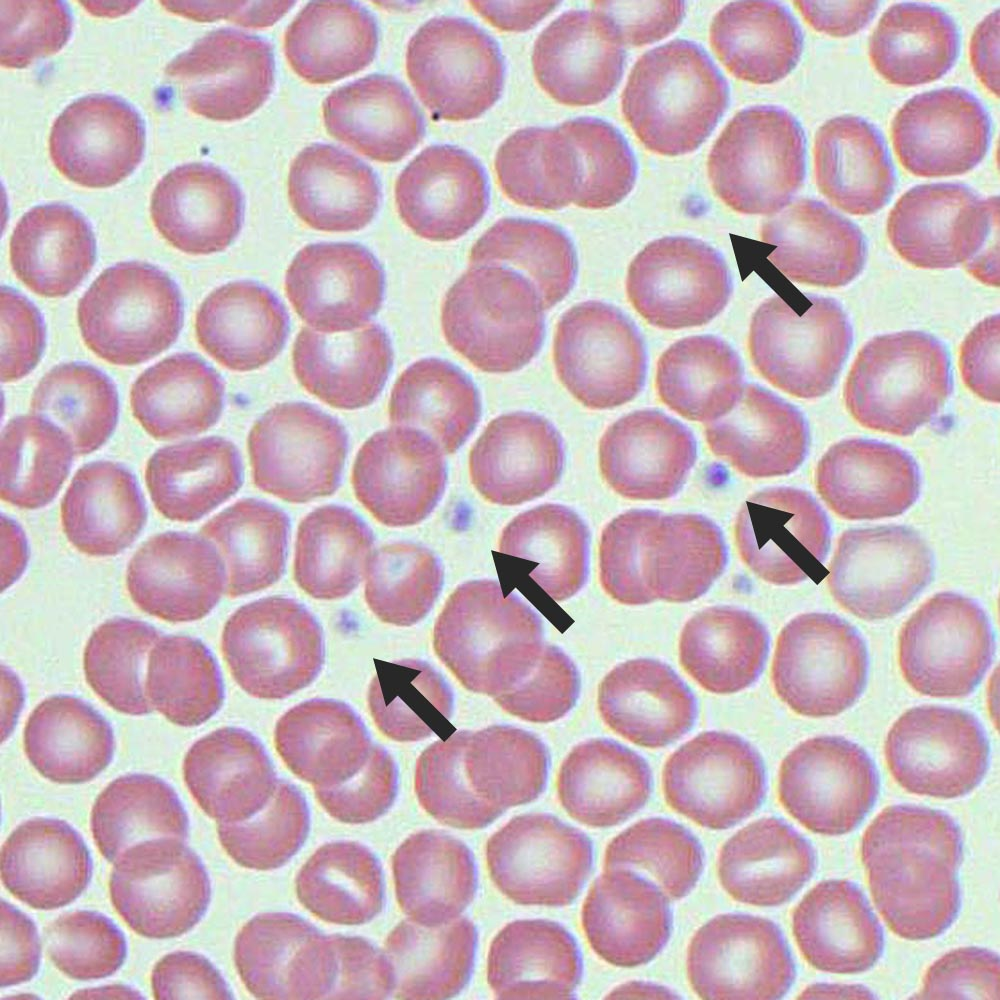
\includegraphics[width = 3.1in, height = 2.5in]{../images/platelets.jpg}}}
    \caption{Platelets}
\end{figure}


\newpage

\vspace*{\fill}
\begin{center}
    {\color{Black} \rule{\linewidth}{1.2mm} }\\
\vspace{0.25in}
 {\centering\fontsize{30}{40}{\bfseries{\color{Black}{\scshape{Chapitre I : Etat de l'art}}}}}
\vspace{0.35in}\\
    {\color{Black} \rule{\linewidth}{1.2mm} }
\end{center}
\vspace*{\fill}
\addcontentsline{toc}{chapter}{\color{Black}{Chapitre I : Etat de l'art}}
\setcounter{section}{0}

\newpage

\section{Introduction}
\vspace{0.2in}
\hspace*{0.16in}

\section{Related Work}
\vspace{0.2in}
\hspace*{0.16in}
Blood cell segmentation is the extraction of different blood cells from microscopic images. Blood cell counting is the process of counting the detected blood cells after segmentation. Many researchers have implemented methods for segmentation and counting of blood cells.\\

V.KIMBAHUNE and al \textsuperscript{\cite{V.KIMBAHUNE}} have developed a method for segmenting and counting red blood cells (RBC) and white blood cells (WBC).
segmentation is done using Pulse-Coupled Neural Network (PCNN) and square tracing algorithm for countour tracing after de-noising it with PCNN + median filter, the counting is performed by scaning the image and using edge detection method. this method gave good results compared to state of art methods.

Bhavnani and al \textsuperscript{\cite{bhavnani2016segmentation}} have developed a method for segmenting and counting RBC (red blood cells), WBC (White blood cells) and platelets which is also called complete blood count (CBC), by using Otsu’s thresholding and morphological operations as a segmentation method, and for counting the are preforming a comparison between two methods: the watershed algorithm and Circular Hough Transform. the CHT method is the best in terms of accuracy but it has some weaknesses with overlaping cells and morphological abnormalities.

Carlos X. Hern{\'{a}}ndez et al \textsuperscript{\cite{DBLP:journals/corr/abs-1802-10548}} have implemented a convolutional neural network (CNN) using a feature pyramid network combined with a VGG style neural network for segmenting and counting of cells in a given microscopy image which achieved a relatively good accuracy of 95\% but with some failure cases such as: High cell overlap, Irregular cell shapes and bad focal planes.

K. Sudha and P. Geetha \textsuperscript{\cite{SUDHA2020639}} have developed a two stage framework which will segment the leukocytes (a type of WBC) with an edge strength-based Grabcut method as a first stage, in the second stage will count the cells using the novel gradient circular hough transform (GCHT) method. the new GCHT method can segment touched cells and even overlapped cells.

Overton, Toyah and Tucker, Allan \textsuperscript{\cite{10.1007/978-3-030-44584-3_31}} have developed method about segmentation and counting IDP(Internally Displaced people) and erythrocytes (red blood cells) using DO-U-Net (Dual Output U-Net) which outputs a segmentation mask and an edge mask then they substract them to get rid of the overlapping and the touching problem, the model trains on extremely small datasets (10 images) and gives a high segmentation accuracy, for the IDP they had 98.69\% for fixed resolution images and 94.66\% for scale-invariant satellite images.

\section{Conclusion}
\vspace{0.1in}
\hspace*{0.16in}


\newpage

\vspace*{\fill}
\begin{center}
    {\color{Black} \rule{\linewidth}{1.2mm} }\\
\vspace{0.25in}
    {\centering\fontsize{30}{40}{\bfseries{\color{Black}{\scshape{Chapter II : Dataset Collection}}}}}
\vspace{0.35in}\\
    {\color{Black} \rule{\linewidth}{1.2mm} }
\end{center}
\vspace*{\fill}
\addcontentsline{toc}{chapter}{\color{Black}{Chapter II : Dataset Collection}}
\setcounter{section}{0}

\newpage

% \thispagestyle{empty}
\vspace*{\fill}
\begin{center}
    {\color{Black} \rule{\linewidth}{1.2mm} }\\
\vspace{0.25in}
 {\centering\fontsize{30}{40}{\bfseries{\color{Black}{\scshape{Chapter II : State of the art}}}}}
\vspace{0.35in}\\
    {\color{Black} \rule{\linewidth}{1.2mm} }
\end{center}
\vspace*{\fill}
\addcontentsline{toc}{chapter}{\color{Black}{Chapter II : State of the art}}
\setcounter{section}{0}

\newpage

\section{Introduction}
\vspace{0.2in}
\hspace{\parindent}
Blood cell segmentation is the extraction of different blood cells from microscopic images. Blood cell counting is the process of counting the detected blood cells after segmentation. Many researchers have implemented methods for segmentation and counting of blood cells using different approaches. In this section we first explore the used databases in their research and then present the methods according to the segmentation approach.

\section{DataSet Collections}
In this section we are comparing between the databases and their annotations that are available to pick the best database that will fit our problem. We can see that there is a lot of datasets which are created to attack a specific sets of problems, we can see below all available datasets:
%we will try to find the best dataset that will help us with our problem, by performing a comparison between all the available datasets and their annotations, we can see that there is a lot of datasets which are created to attack a specific sets of problems, we can see below all available datasets:

\subsection{ALL-IDB}
\hspace{\parindent}
ALL-IDB (Acute Lymphoblastic Leukemia Image Database for Image Processing) \textsuperscript{\cite{labati2011all}} is a public and free dataset, specifically designed for the evaluation and the comparison of algorithms for segmentation and image classification. The database focus on Acute Lymphoblastic Leukemia (ALL), Acute is a type of blood cancer that starts in white blood cells in bone marrow, the soft inner part of bones. It develops from immature lymphocytes, a kind of white blood cell that’s key to immune system.\textsuperscript{\cite{Annie_Stuart_What_2022_webmd}}.\

Each image in the dataset, Contains classification/position of ALL lymphoblasts is provided by expert oncologists. A lymphoblast is a modified naive lymphocyte with altered cell morphology. It occurs when the lymphocyte is activated by an antigen.\

The images of the dataset has been captured with an optical laboratory microscope coupled with a Canon PowerShot G5 camera. All images are in JPG format with 24 bit color depth, resolution 2592 x 1944. the ALL-IDB divides on two Datasets ALL-IDB1 and ALL-IDB2.\

\subsection{Dataset ALL-IDB1}
\hspace{\parindent}
The ALL-IDB1 can be used for segmentation or classification with image processing methods or Artificial intelligence models. The dataset is composed of 108 images collected during September, 2005. It contains about 39000 blood elements, where the lymphocytes has been labeled by expert oncologists.

\begin{figure}[H]
\centering
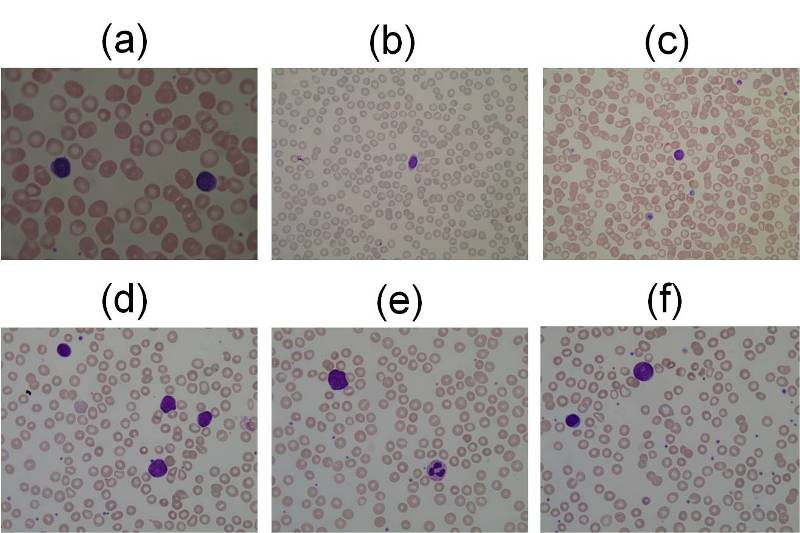
\includegraphics[width=5.8in]{../images/ALLIDB1.jpg}
\caption{Examples of the images contained in ALL-IDB1: healthy cells from non-ALL patients (a,b,c), probable lymphoblasts from ALL patients (d,e,f). }
\end{figure}

\textbf{annotation:} input image ''Im006\_1.jpg'' (a) and the related classification file ''Im006\_1.xyc'' reporting the coordinates of the centroids of probable ALL lymphoblasts (b).

\begin{figure}[H]
\begin{minipage}[b]{0.35\linewidth}
\centering
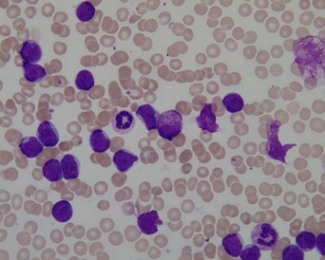
\includegraphics[width=55mm]{../images/Im006_1.jpg}
\subcaption{Im006\_1.jpg}
\label{fig:Im006.jpg}
\end{minipage}
\hfill
\begin{minipage}[b]{0.3\linewidth}
\centering
\lstinputlisting[breaklines]{../images/Im006\_1.xyc}
\subcaption{Im006\_1.xyc}
\label{fig:Im006.xyc}
\end{minipage}

\begin{minipage}[b]{0.35\linewidth}
\centering
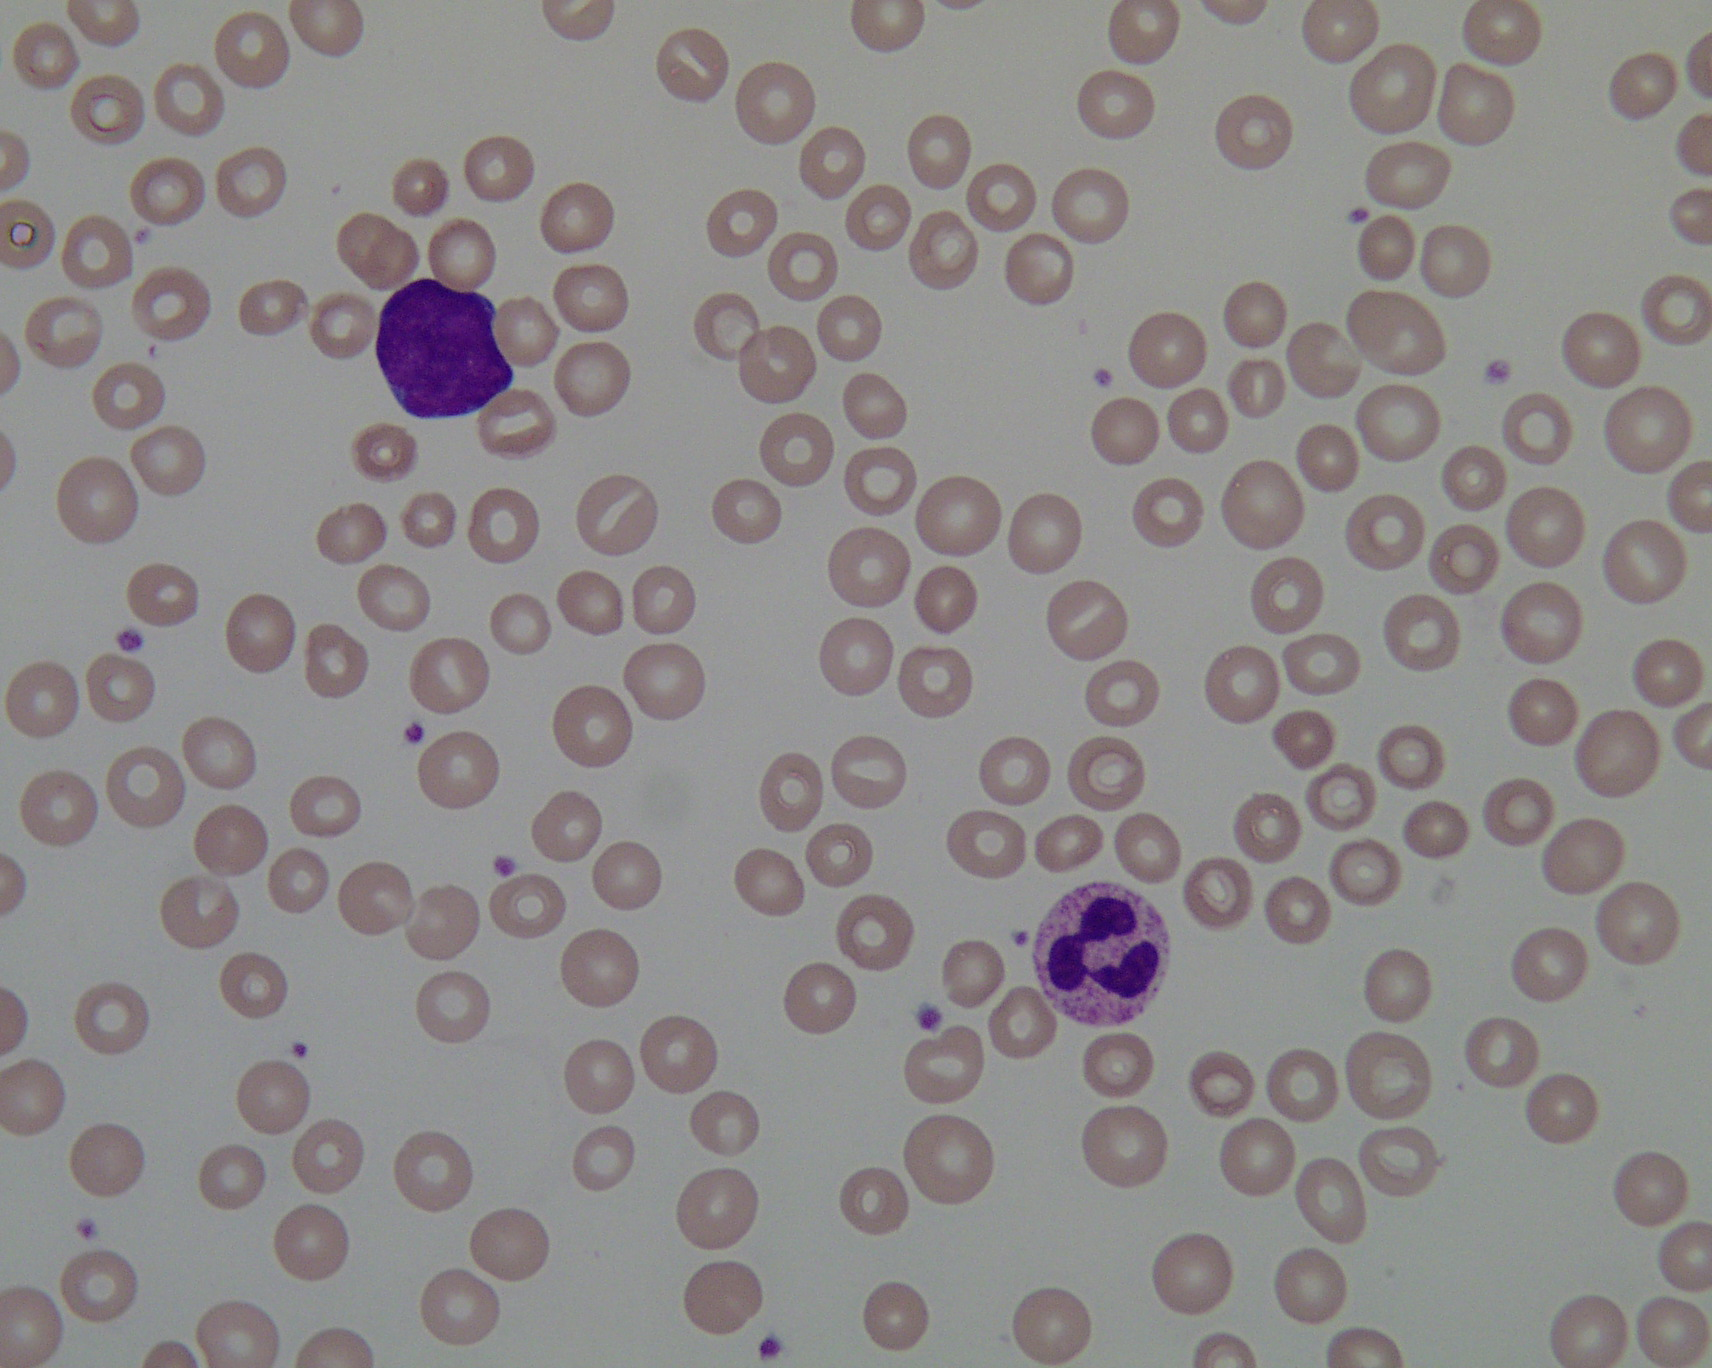
\includegraphics[width=55mm]{../images/Im033_1.jpg}
\subcaption{Im033\_1.jpg}
\label{fig:Im033.jpg}
\end{minipage}
\hfill
\begin{minipage}[b]{0.3\linewidth}
\centering
\lstinputlisting[breaklines]{../images/Im033\_1.xyc}
\subcaption{Im033\_1.xyc}
\label{fig:Im033.xyc}
\end{minipage}
\caption{Sample data from the ALL-IDB1 Database}
\end{figure}

The ALL-IDB1 image files are named with the notation ImXXX\_Y.jpg where XXX is a 3-digit integer counter and Y is a boolean digit equal to 0 if no blast cells are present, and equal to 1 if at least one blast cell is present in the image. All images labeled with Y=0 are from for healthy individuals, and all images labeled with Y=1 are from ALL patients. Each image file ImXXX\_Y.jpg (figure \ref{fig:Im006.jpg}, \ref{fig:Im033.jpg}) is associated with a text file ImXXX\_Y.xyc (figure \ref{fig:Im006.xyc}, \ref{fig:Im033.xyc}) reporting the coordinates of the centroids of the blast cells, if any.\\

If we plot the coordinates in the Img006\_1.xyc (figure \ref{fig:Im006.jpg}) file on the image Im006\_1.jpg (figure \ref{fig:Im006.xyc}) we get the figure \ref{fig:Im006.xyc.jpg}



\begin{figure}[H]
\centering
    \fbox{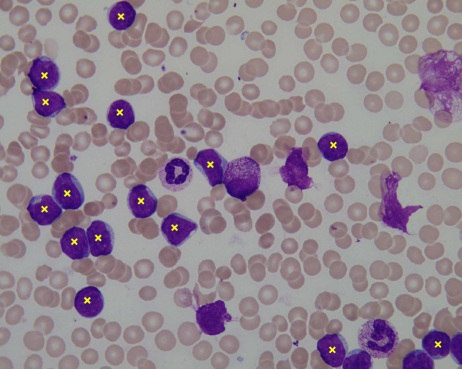
\includegraphics[width = 4in]{../images/img006.xyc.jpg}}
\caption{coordinates from Img006\_1.xyc plotted on Img006\_1.jpg}
\label{fig:Im006.xyc.jpg}
\end{figure}

\subsubsection{Dataset ALL-IDB1}
\hspace{\parindent}
This dataset has been created for testing the performances of classification systems. where the dataset has no segmentation information it contains only one information which is the presence of ALL lymphoblasts, the dataset is a collection of cropped area of interest of normal and blast cells that belongs to the ALL-IDB1 dataset as we can see in figure \ref{fig:ALL-IDB2}

\begin{figure}[H]
\centering
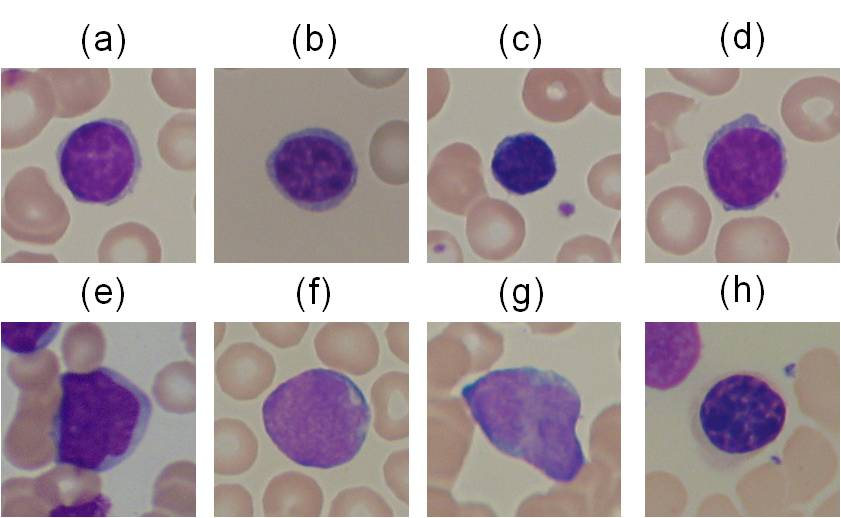
\includegraphics{../images/ALL-IDB2.jpg}
\caption{Examples of the images contained in ALL-IDB2: healthy cells from non-ALL patients (a-d), probable lymphoblasts from ALL patients (e-h).}
\label{fig:ALL-IDB2}
\end{figure}

\vspace{-0.14in}

The annotation of ALL-IDB2 is similar to the ALL-IDB1 but with no centroid coordinates. The ALL-IDB2 image files are named with the notation ImXXX\_Y.jpg where XXX is a progressive 3-digit integer and Y is a Boolean digit equal to 0 if the cell placed in the center of the image is not a blast cell, and equal to 1 if the cell placed in the center of the image is a blast cell. all images labeled with Y=0 are from for healthy individuals, and all images labeled with Y=1 are from ALL patients. 

\subsection{Broad Bio-image Benchmark Collection}
\hspace{\parindent}
The Broad Bio-image Benchmark Collection (BBBC) is a collection of freely downloadable microscopy image sets, cited in 450+ studies. In addition to the images themselves, each set includes a description of the biological application and some type of "ground truth" (expected results) \textsuperscript{\cite{ljosa2012annotated}}. The BBBC is organized by the Broad Institute's Imaging Platform.\

The dataset contains 54 image collections of various cell types, each collection has at least one of 6 ground truth types such as cell count, foreground / background, outlines of objects, biological labels, location and bounding boxes. in the sections below we describe each ground truth:

\subsubsection{Cell counts}
\hspace{\parindent}
In this case, the ground truth consists of the number of cells (or other objects) in each image, as counted by one or more humans. for example in BBBC1(Human HT29 colon-cancer cells) we have an image in figure \ref{fig:BBBC1} with the labels file in figure \ref{fig:BBBC001_Counts}:

\begin{figure}[H]
\begin{minipage}[c]{\linewidth}
\centering

\includegraphics[width = 2.2in]{../images/AS_09125_050118150001_A03f05d0.jpg}
\subcaption{AS\_09125\_050118150001\_A03f05d0.jpg}
\label{fig:BBBC1}
\end{minipage}

\begin{minipage}[c]{\linewidth}
\centering
\lstinputlisting[breaklines]{../images/BBBC001_v1_counts.txt}
\subcaption{BBBC001\_v1\_counts.txt}
\label{fig:BBBC001_Counts}
\end{minipage}
\caption{Sample data from the BBBC1 Database with counts Ground truth}
\end{figure}

in the figure \ref{fig:BBBC001_Counts} we can see the two counts performed by two experts, for the image \ref{fig:BBBC1} the first expert have found 241 cells but the second one found 257 cells.

\subsubsection{Foreground and background}
\hspace{\parindent}
In this case, a human produces a binary (black and white but in some cases thy use other colors) image the same size as the original image. Pixels that belong to the foreground (i.e., the cells or other objects) are white, and pixels that belong to the background are black. in the example below (figure \ref{fig:BBBC004_img} and \ref{fig:BBBC004_F}) we can see the image and the corresponding mask where the cells colored with blue and the background with black.

\begin{figure}[H]
\begin{minipage}[c]{0.4\linewidth}
\centering
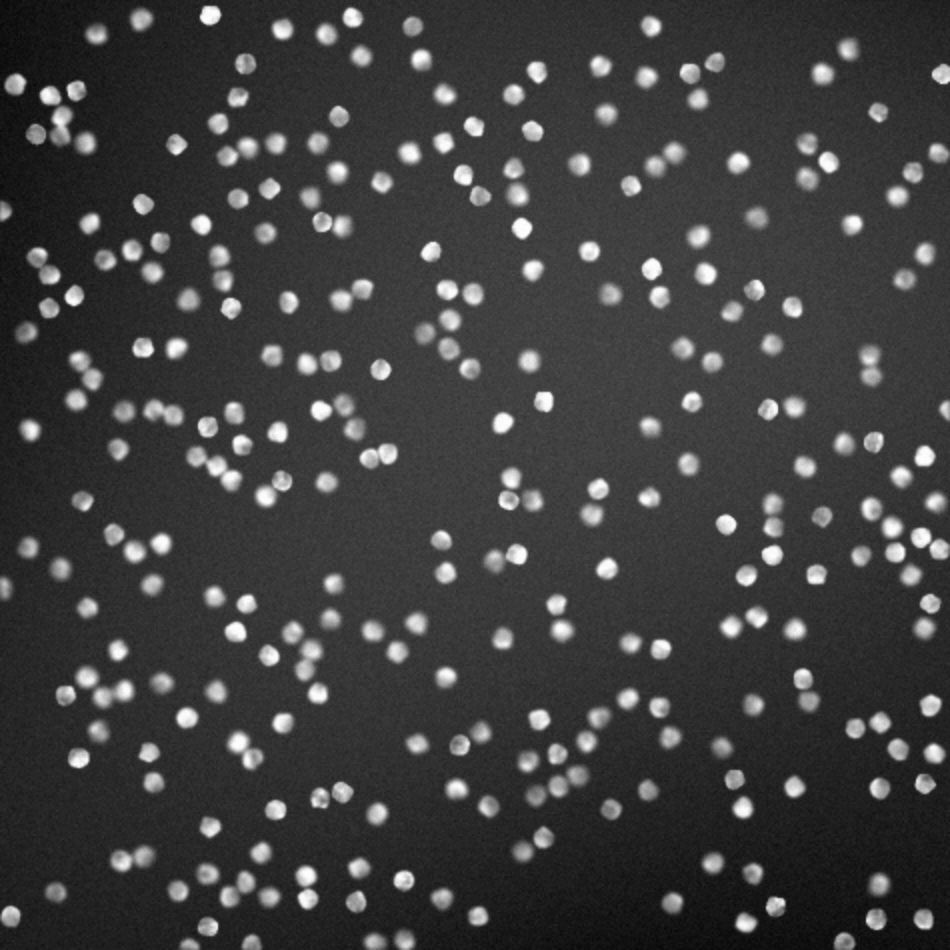
\includegraphics[width=50mm]{../images/BBBC4-1.jpg}
\subcaption{2Gray1.tif (image)}
\label{fig:BBBC004_img}
\end{minipage}
\hfill
\begin{minipage}[c]{0.4\linewidth}
\centering
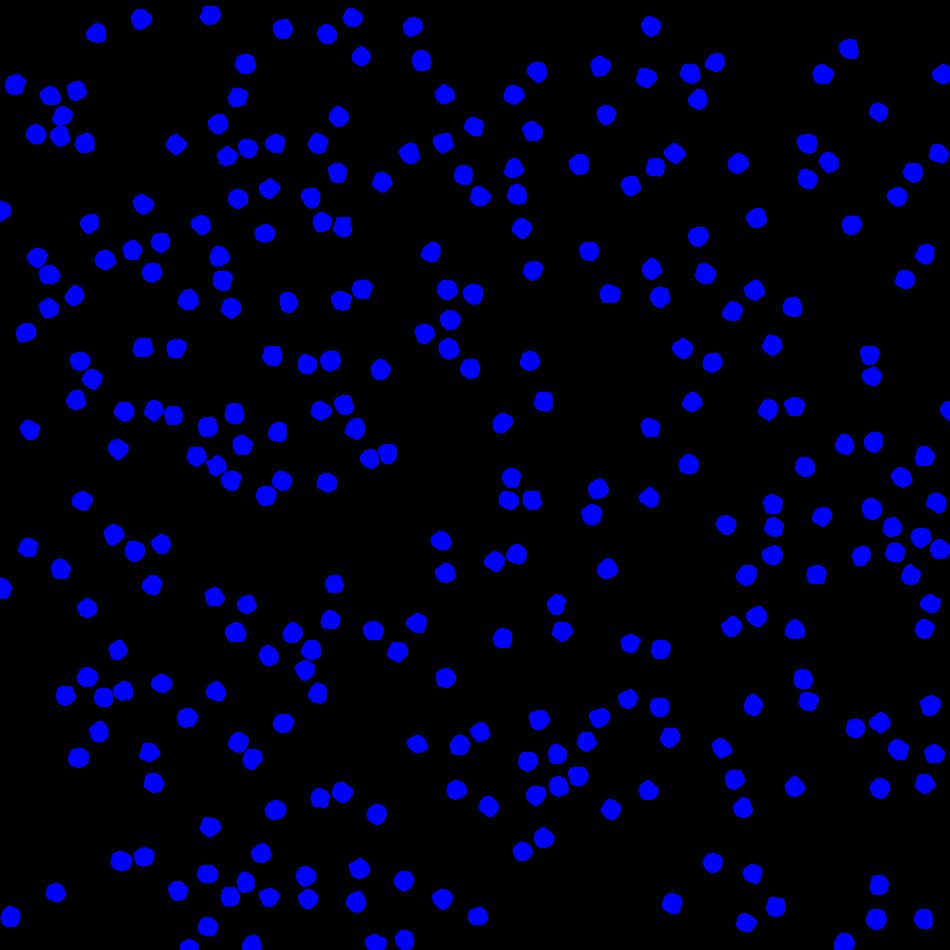
\includegraphics[width=50mm]{../images/BBBC4-1-F.jpg}
\subcaption{1.tif (mask)}
\label{fig:BBBC004_F}
\end{minipage}
\caption{Sample data from the BBBC4 Database with mask as ground truth}
\end{figure}

\subsubsection{Outlines of individual objects}
\hspace{\parindent}
In this case, a human outlines each cell in the image in order to indicate which pixels belong to which cell. The ground truth is provided as binary images, with black outlines on a white background.

\begin{figure}[H]
\begin{minipage}[c]{0.4\linewidth}
\centering
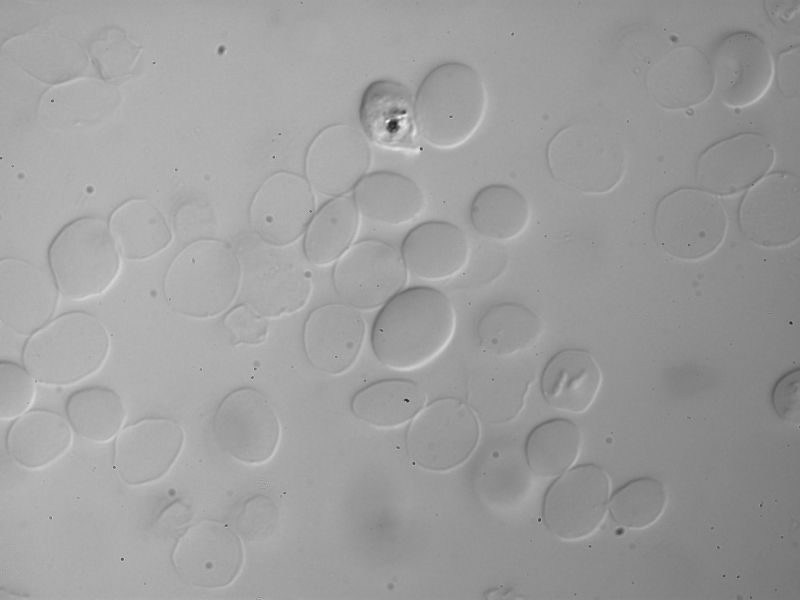
\includegraphics[width=50mm]{../images/48hr-001-DIC.jpg}
\subcaption{48hr-001-DIC.jpg (image)}
\label{fig:BBBC009_img}
\end{minipage}
\hfill
\begin{minipage}[c]{0.4\linewidth}
\centering
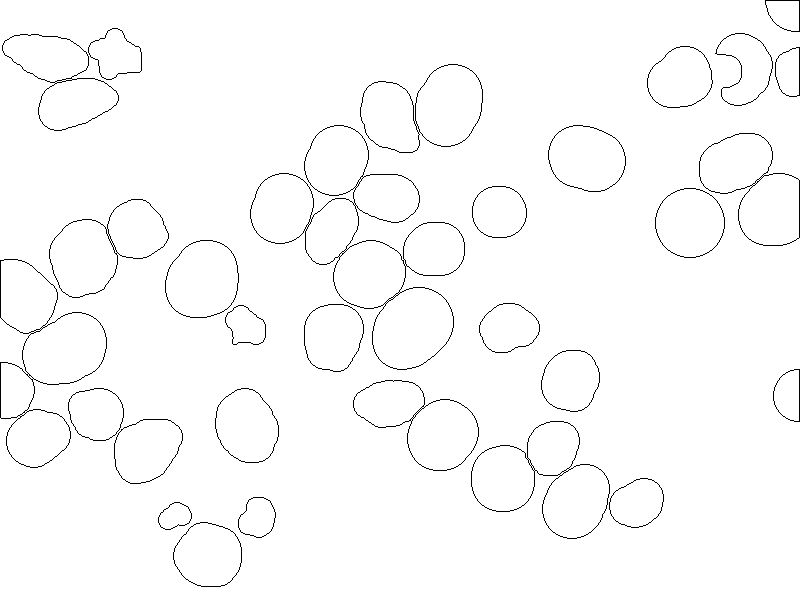
\includegraphics[width=50mm]{../images/48hr-001-DIC_.jpg}
\subcaption{48hr-001-DIC.jpg (edge mask)}
\label{fig:BBBC009_O}
\end{minipage}
\caption{Sample data from the BBBC9 Database with edge mask (outlines) as ground truth}
\end{figure}

\subsubsection{Biological labels}
\hspace{\parindent}
In these cases, the experiments have been prepared with control samples for which we know the expected biological result. The types of controls that are available dictate the type of statistic that can be calculated.

\subsubsection{Location}
\hspace{\parindent}
In this case, the ground truth consists of the X, Y, and optionally Z location of objects (typically their centroids similar to ALL-IDB1 Annotation \ref{fig:Im006.xyc.jpg}) .

\subsubsection{Bounding Boxes}
\hspace{\parindent}
Bounding boxes are rectangles completely enclosing an object.

\vspace{-0.1in}

\subsection{WBC Image Dataset : Fast and Robust Segmentation of White Blood Cell Images by Self-supervised Learning}
\hspace{\parindent}
This is two datasets of white blood cell (WBC) images used for “Fast and Robust Segmentation of White Blood Cell Images by Self-supervised Learning”, which can be used to evaluate cell image segmentation methods \textsuperscript{\cite{Zheng2018}}.\
This collection contains two datasets different from each other in terms of the image color, cell shape, background, etc. The ground truth segmentation results are manually sketched by domain experts, where the nuclei, cytoplasms and background including red blood cells are marked in white, gray and black respectively. 

\subsubsection{Dataset 1}
\hspace{\parindent}
Was obtained from Jiangxi Tecom Science Corporation \textsuperscript{\cite{2022_tecom-cn}}, China. It contains three hundred 120×120 images of WBCs and their color depth is 24 bits. The images were taken by a Motic Moticam Pro 252A optical microscope camera with a N800-D motorized auto-focus microscope.

\begin{figure}[H]
\centering
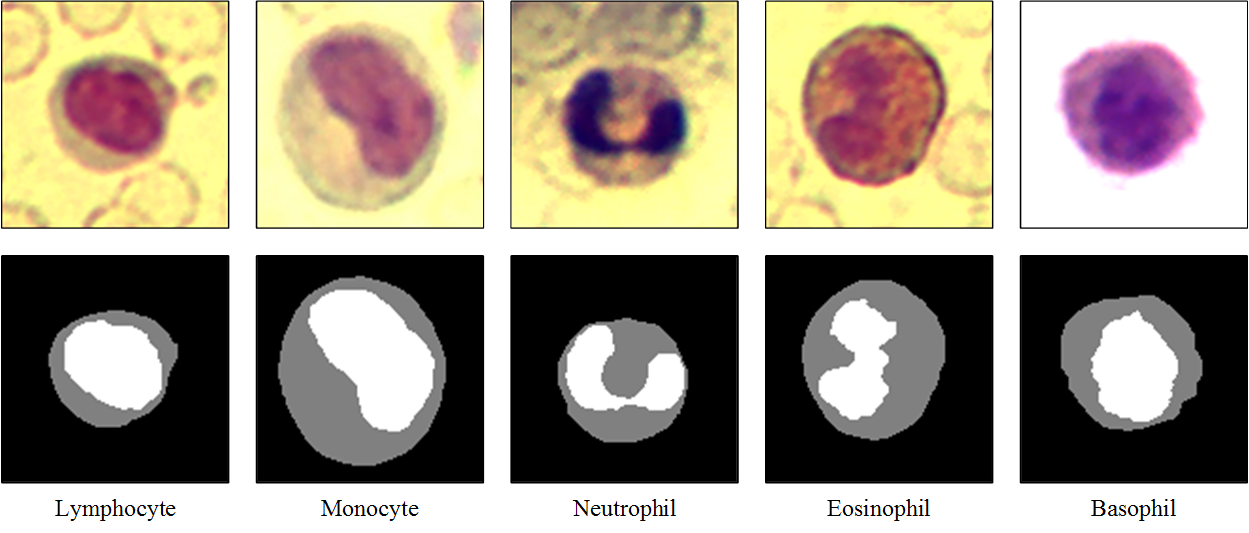
\includegraphics[width=5.2in]{../images/WBC_Dataset1.png}
\caption{Sample data from WBC\_Segmentaion Dataset 1}
\label{fig:WBC_Dataset1_sample}
\end{figure}

\subsubsection{Dataset 2}
Consists of one hundred 300×300 color images, which were collected from the Cella-Vision blog \textsuperscript{\cite{2022_cellavision}}. The cell images are generally purple and may contain many red blood cells around the white blood cells.

\begin{figure}[H]
\centering
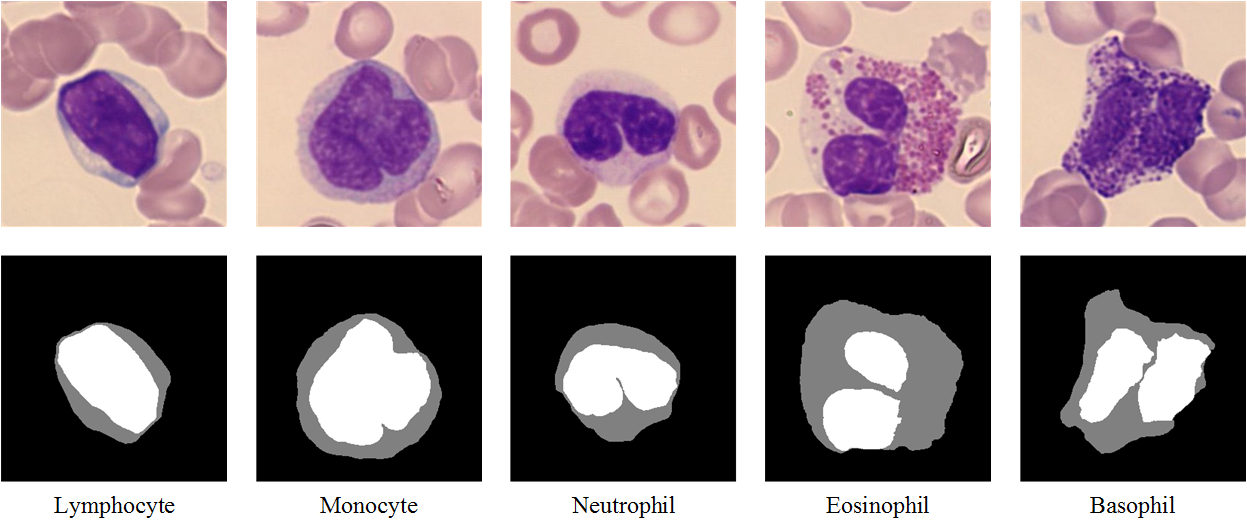
\includegraphics[width=5.2in]{../images/WBC_Dataset2.png}
\caption{Sample data from WBC\_Segmentaion Dataset 2}
\label{fig:WBC_Dataset2_sample}
\end{figure}

\subsection{Annotation}
\hspace{\parindent}
The class labels of each image in Dataset 1 and Dataset 2 are stored in csv files. The labels (1- 5) represent neutrophil, lymphocyte, monocyte, eosinophil and basophil, respectively.


\subsection{A large dataset of white blood cells containing cell locations and types, along with segmented nuclei and cytoplasm}
\hspace{\parindent}
The database is provided by \href{https://raabindata.com/free-data/#double-labeled-cropped-cells}{RabinData} and \textsuperscript{\cite{Kouzehkanan2022}} which divides on two separate datasets:

\subsubsection{Raabin-WBC Data}
\hspace{\parindent}
Contains 4 sub-Datasets:
\begin{itemize}
    \item \textbf{Double-labeled cropped cells} : Double-labeled cropped cells are also provided containing only five main classes including mature neutrophils, lymphocytes (small and large), eosinophils, monocytes, and basophils. 
    \item \textbf{Nucleus\_cytoplasm\_Ground truths} : in this sub-Dataset they prepared the ground truths of the cytoplasm and the nucleus for a proper number of cropped white blood cells. For this purpose, 1145 cropped images including 242 lymphocytes, 242 monocytes, 242 neutrophils, 201 eosinophils, and 218 basophils were randomly selected, and their ground truths were extracted by an expert.
    \item \textbf{Microscopic images were taken by the Olympus CX18 microscope and the Samsung Galaxy S5 camera and the 4th database with contain images taken by Zeiss microscope and the LG G3 camera } : in these two sub-Datasets. Corresponding to each microscopic image, a dictionary (json format) file containing the following information about that image was provided:
    \begin{itemize}
        \item Information about the blood elements in the image including their coordinates and labels.
        \item Information about the blood smears including staining method and the type of the disease.
        \item Information about the microscope includes the type of microscope and its magnification size.
        \item The type of camera used.
    \end{itemize}
\end{itemize}

\subsubsection{Raabin-Leukemia Data}
\hspace{\parindent}
Contains 4 sub-Datasets:
\begin{itemize}
    \item \textbf{Acute Lymphoblastic Leukemia}
    \item \textbf{Acute Myeloblastic Leukemia} 
    \item \textbf{Chronic Lymphocytic Leukemia}
    \item \textbf{Chronic Myelogenous Leukemia}
\end{itemize}
In each of these sub-Dataset, All samples were taken from patients who had referred to our collaborator medical laboratory (Takht-e Tavous Laboratory in Tehran, Iran). It should be notices Zeiss microscope and LG J3 smartphone camera had been used for imaging.

\subsection{BCCD}
\hspace{\parindent}
BCCD (Blood Cell Count and Detection) Dataset is a small-scale dataset for blood cells detection. The dataset contains a total of 364 (640x480) jpeg images with their annotations. The original data and annotations are from \href{https://github.com/cosmicad/dataset}{cosmicad} and \href{https://github.com/akshaylamba/all_CELL_data}{akshaylamba}.\\
In this project, the Faster R-CNN algorithm from keras-frcnn for Object Detection is used. From this dataset, nicolaschen1 developed two Python scripts to make preparation data (CSV file and images) for recognition of abnormalities in blood cells on medical images.

\begin{figure}[H]
\centering
    \fbox{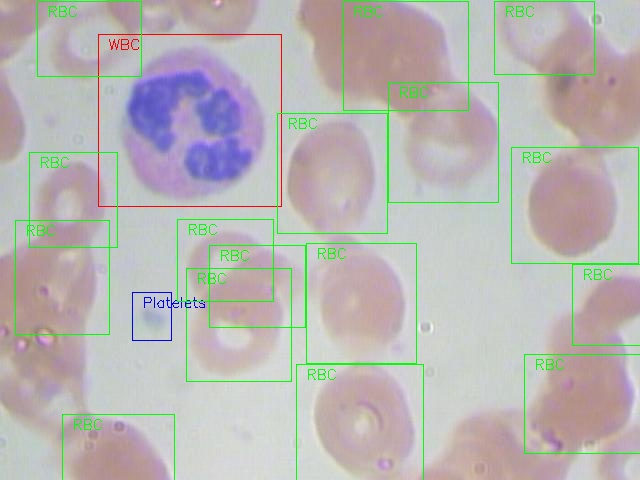
\includegraphics[width=4.2in]{../images/BBCD1.jpg}}
\caption{Sample data from BBCD}
\label{fig:BBCD1}
\end{figure}

In this database they use bounding boxes to locate the cells and each bounding box has the type of cell RBC or WBC and Platelets. they are using the VOC format as a database architecture.

\subsection{Dataset collections resume}
\hspace{\parindent}

\begin{table}[H]
\centering
\resizebox{\textwidth}{!}{%
\begin{tabular}{|c|c|ccc|c|c|}
\hline
\cellcolor[HTML]{FFFFFF}\textbf{\begin{tabular}[c]{@{}c@{}}Dataset\\ Name\end{tabular}} &
  \cellcolor[HTML]{FFFFFF}\textbf{\begin{tabular}[c]{@{}c@{}}Dataset\\ Size\end{tabular}} &
  \multicolumn{3}{c|}{\textbf{\begin{tabular}[c]{@{}c@{}}Type of cells\\ (RBC, WBC, Platelets)\end{tabular}}} &
  \cellcolor[HTML]{FFFFFF}\textbf{Type of annotation} &
  \cellcolor[HTML]{FFFFFF}\textbf{Description} \\ \hline
\cellcolor[HTML]{FFFFFF}ALL-IDB \textsuperscript{\cite{pm77-2n23-20}}&
  \cellcolor[HTML]{FFFFFF}108 &
  \multicolumn{1}{c|}{108 masks / 13 edges} &
  \multicolumn{1}{c|}{108 masks} &
  108 masks&
  \cellcolor[HTML]{FFFFFF}\begin{tabular}[c]{@{}c@{}}Location \\ (Centroid of cells)\end{tabular} &
  \cellcolor[HTML]{FFFFFF}\begin{tabular}[c]{@{}c@{}}Acute Lymphoblastic\\ Leukemia Image Database\\ for Image Processing\end{tabular} \\ \hline
\cellcolor[HTML]{FFFFFF}BBBC \textsuperscript{\cite{ljosa2012annotated}} &
  \cellcolor[HTML]{FFFFFF}Lots of subdatasets &
  \multicolumn{1}{c|}{X} &
  \multicolumn{1}{c|}{X} &
  X &
  \cellcolor[HTML]{FFFFFF}\begin{tabular}[c]{@{}c@{}}All types of\\ annotations\end{tabular} &
  \cellcolor[HTML]{FFFFFF}\begin{tabular}[c]{@{}c@{}}Broad Bioimage Benchmark\\ Collection\end{tabular} \\ \hline
\cellcolor[HTML]{FFFFFF}WBC Image Dataset &
  \cellcolor[HTML]{FFFFFF}400 &
  \multicolumn{1}{c|}{} &
  \multicolumn{1}{c|}{X} &
   &
  \cellcolor[HTML]{FFFFFF}\begin{tabular}[c]{@{}c@{}}Foreground and\\ Background (mask)\end{tabular} &
  \cellcolor[HTML]{FFFFFF}\begin{tabular}[c]{@{}c@{}}WBC Image Dataset : \\ Fast and Robust Segmentation\\ of White Blood Cell Images\\ by Self-supervized Learning\end{tabular} \\ \hline
    BCCD \textsuperscript{\cite{BCCD_Dataset}} &
  364 &
  \multicolumn{1}{c|}{} &
  \multicolumn{1}{c|}{x} &
   &
  Bounding boxes &
  Blood Cell Count and Detection \\ \hline
\end{tabular}%
}
\caption{Table that resumes datasets mentioned above}
\label{Table that resumes datasets mentioned above}
\end{table}


\section{Computer-assisted blood cell segmentation and counting review}

\subsection{Image Processing Approaches}
\hspace{\parindent}
Bhavnani et al. \textsuperscript{\cite{bhavnani2016segmentation}} have developed a method for segmenting and counting RBC (red blood cells), WBC (White blood cells) and platelets which is also called complete blood count (CBC), by using Otsu’s thresholding and morphological operations as a segmentation method, and for counting the are preforming a comparison between two methods: the watershed algorithm and Circular Hough Transform. The model takes an RGB image as an input apply some processing steps then uses Otsu's thresholding to extract RBC and WBC separately with different threshold values then apply the two algorithm to compare the results, the model has no image size constraint because it's based only on image processing techniques and needs a small database to select the threshold values for RBC and WBC in this article they used 20 images. In the Experiment phase they used ALLIDB Database which contains 108 images with 1712x1368 and 2592x1944 resolution.The CHT method is the best in terms of accuracy with 92.67\% but it has some weaknesses with overlapping cells and morphological abnormalities. In the other side the watershed method which is a little bit adapted with overlapping and touching cells had an accuracy of 91.07\%.\

Guiliang, FENG et al. \textsuperscript{\cite{guiliang2016microscopic}} have a developed an algorithm that segments and counts cell images based on image definition, a Discrete Cosine Transform (DCT) is applied, which is proposed by N. Ahmed and Rao in 1974 \textsuperscript{\cite{ahmed1974discrete}}. Instead of the traditional watershed approach, the DCT method showed better results in comparison.\

However, there is a drawback to this approach, because this algorithm depends on image definition it relies on well focused images, consequently, when the images are out of focus the segmentation and counting is not reliable. But despite that drawback, it achieved a relatively high accuracy of over 90\% which is better that the watershed method.\\

K. Sudha and P. Geetha \textsuperscript{\cite{SUDHA2020639}} have developed a two stage framework which will segment the leukocytes (a type of WBC) with an edge strength-based Grabcut method as a first stage, in the second stage will count the cells using the novel gradient circular hough transform (GCHT) method. the model takes and RGB image convert it to HSV color space to extract the S component where the WBCs are more clear then applies the edge strength-based location detection the results are fed to fine segmentation using Grabcut Algorithm which will output the edge segmentation mask, for the counting the mask will be fed to the proposed GCHT Algorithm. In the experiments phase they used ALL-IDB \textsuperscript{\cite{labati2011all}} and Cellavision \textsuperscript{\cite{Zheng2018}} datasets, after resizing the images to 256x256.\\
After the experiments the proposed method had reached an average segmentation accuracy of 99.32\% and a counting accuracy of 97.3\%.\\
The new GCHT method can segment touched cells and even overlapped cells.

\subsection{Machine Learning Approaches}
\hspace{\parindent}
Kimbahune et al. \textsuperscript{\cite{kimbahune2011blood}} have developed a method for segmenting and counting red blood cells (RBC) and white blood cells (WBC).
segmentation is done using Pulse-Coupled Neural Network (PCNN) and square tracing algorithm for contour tracing after de-noising it with PCNN combined with median filter, the counting is performed by scanning the image and using edge detection methods as square tracing algorithm. this method gave good results compared to state of art methods.\\
%this kimbahune article they didn't give any info about the database or the experimental results 

Carlos X. Hern{\'{a}}ndez et al. \textsuperscript{\cite{DBLP:journals/corr/abs-1802-10548}} have implemented a convolutional neural network (CNN) using a feature pyramid network (FPN) combined with a VGG style neural network for segmenting and counting of cells in a given microscopy image.\
The dataset they used is BBBC005 \textsuperscript{\cite{ljosa2012annotated}} from Broad Institute's Bio-image Benchmark Collection, which consists of 9600 images and each image is 696x520 pixels but they were scaled down to 256x192 for the purposes of their experiment.\

Out of the total 9600 images only 600 of the images which have a corresponding mask were used for the FPN training. And 100 of those were used for fast prototyping and a standard of 80-20 train/test split for the final models.\
On the other hand, the full 9600 images were used for the VGG network.
This approach achieved a relatively good accuracy of 81.75\% but with some failure cases such as:\
%the accuracy is calculated manually from the given results in the article
% 100 - (rmspe = np.sqrt(np.mean(np.square(((y_true - y_pred) / y_true)), axis=0)))

\begin{itemize}
  \item High cell overlap
  \item Irregular cell shapes
  \item bad focal planes.
\end{itemize}

Tran, Thanh and Minh et al. \textsuperscript{\cite{tran2019blood}} have developed a method for segmenting and counting RBC and WBCs by using the SegNet model initialised with weights from a pre-trained VGG-16 model, for the counting they first apply Distance transform with 4 different distance metrics, then they apply binary dilation. At the End, they apply the connected component labeling algorithm to count the number of separated cells in images mask. for the training they used 42 images from ALL-IDB1 \textsuperscript{\cite{labati2011all}} after they cropped them to decrease the computation time and memory usage and reduce the number of RBC compared to WBC the result images have a resolution of 360*480*3 (RGB), they used 29 images for training and 13 for testing ,the model had a segmentation accuracy of 89\% and counting accuracy of 93.3\% on RBC and accuracy of 100\% on WBC with the testing database which has the cropped images of RBC and WBC.\

On the first database with cropped images they had only few WBC but in this second database they have more WBC , the database 2 contains 108 only WBC images with the same size of database 1 360*480*3, they augmented the training dataset from 76 to 380 and used 32 images for testing, this second model focus only on the WBC which will increase the segmentation accuracy to 98.5\%, and have a counting accuracy of 97.29\%. The counting accuracy have decreased because of the clumped cells which is the weakness of this model.\\

Yan Kong et al. \textsuperscript{\cite{Kong:20}} have developed a two-stage framework using parallel modified U-Nets together with seed guided water-mesh algorithm for automatic segmentation and yeast cells counting which is used to observe the living conditions and survival of yeast cells under experimental conditions.\

The cell images used in this study were captured by Olympus IX83 (Olympus Life Sciences, Tokyo, Japan) inverted microscope. They manually selected 20 raw DIC (differential interference contrast) images which contained a number of yeast cells and the annotations were done manually by laboratory technicians, they then obtain 40 images, 20 masked annotation images and the other 20 is center annotation images of yeast cells.\

After splitting images into tiles of size 224x224 with a step stride of 65 and 33 pixels for the horizontal and vertical direction, respectively. They got 4360 raw image tiles and the corresponding center annotation and masked annotation images, from that set 3310 tiles were randomly selected as the training data set and rest was a validation set.

The raw test DIC images used in this study were sized approximately 1002x1998 pixels, but they were resized into 1092x2084 pixels so that each DIC image could be split into a grid of 8x16 image blocks. The image blocks were then fed into modified U-Net.

This method achieved a precision of over 99.74\% and an average recall rate of 99.35\%. however, there is a limitation using this approach, which is the detection of small objects.\\

Shahzad, Muhammad et al. \textsuperscript{\cite{shahzad2020robust}} have developed a custom convolutional encoder-decoder framework along with VGG-16 as the pixel-level feature extraction model to address the problem of whole-slide cell segmentation using the semantic segmentation approach. Their proposed framework works as follows: First, all the original images along with manually generated ground truth masks of each blood cell type are passed through the pre-processing stage. In the pre-processing stage, pixel-level labeling, RGB to gray-scale conversion of masked image and pixel fusing, and unity mask generation are performed. After that, VGG16 is loaded into the system, which acts as a pre-trained pixel-level feature extraction model. Finally, the training process is initiated on the proposed model.

They used ALL-IDB1 as their baseline dataset which consists of 108 whole-slide blood cell images, 59 (2592x1944) images were from healthy individuals and 49 (1712x1368) images from acute lymphoblastic leukemia (ALL) patients.

This approach achieved a class-wise accuracy of 97.45\%, 93.34\%, and 85.11\% for RBCs, WBCs, and platelets, respectively, while global and mean accuracy remain 97.18\% and 91.96\%, respectively.\\

Overton, Toyah and Tucker, Allan \textsuperscript{\cite{10.1007/978-3-030-44584-3_31}} have developed a method which segments and counts IDP (Internally Displaced people) and erythrocytes (red blood cells) using DO-U-Net (Dual Output U-Net) which outputs a segmentation mask and an edge mask then they subtract them to get rid of the overlapping and the touching problem, the model trains on extremely small datasets (10 images) and gives a high segmentation accuracy, They selected 10 images of 108 from ALL-IDB dataset for training the model, the model takes images with a resolution of 188x188 and outputs a segmentation mask and edge mask of lower resolution 100x100, the experiments results have given an accuracy of 98.31\% on a 5 randomly selected images from ALL-IDB, for the IDP they had 98.69\% for fixed resolution images and 94.66\% for scale-invariant satellite images.\\

Li, Dongming et al. \textsuperscript{\cite{li2021robust}} have developed a method for segmenting blood cells by combining neural ordinary differential equations (NODEs) with U-Net networks to improve the accuracy of image segmentation. In order to study the effect of ODE-solve on the speed and accuracy of the network, the ODE-block module was added to the nine convolutional layers in the U-Net network. Firstly, blood cell images are pre-processed to enhance the contrast between the regions to be segmented; secondly, the same dataset was used for the training set and testing set to test segmentation results. Then they select the location where the ordinary differential equation block (ODE-block) module is added, select the appropriate error tolerance, and balance the calculation time and the segmentation accuracy, in order to exert the best performance.\

Finally, the error tolerance of the ODE-block is adjusted to increase the network depth, and the training NODEs-UNet network model is used for cell image segmentation. 

The experiment dataset for this model was provided by the Center for Medical Image and Signal Processing (MISP) and the Department of Pathology, Isfahan University of Medical Sciences \textsuperscript{\cite{sarrafzadeh2014selection}}. MISP.rar contains 148 clear blood cell smear images with a size of 775x519 pixels. They picked up appropriate areas for convenient network training, then cropped 100 blood cell images with a size of 256x256 pixels by selecting a suitable area. To ensure the accuracy of the training model, they retained 20 images as the testing set and used the remaining 80 images to increase the dataset to 800 by data augmentation. Besides, they used a ratio of 3 : 1 as the training set and the validation set.

Using this approach to segment blood cell images in the testing set, it can achieve 95.3\% pixel accuracy and 90.61\% mean intersection over union. By comparing the U-Net and ResNet networks, the pixel accuracy of this network model is increased by 0.88\% and 0.46\%, respectively, and the mean intersection over union is increased by 2.18\% and 1.13\%, respectively.

\section{Comparative study}

\begin{table}[H]
\centering
\resizebox{\textwidth}{!}{%
\begin{tabular}{|l|cc|c|cc|c|c|}
\hline
\rowcolor[HTML]{FFFFFF} 
\multicolumn{1}{|c|}{\cellcolor[HTML]{FFFFFF}\textbf{Reference}} &
  \multicolumn{1}{c|}{\cellcolor[HTML]{FFFFFF}\textbf{\begin{tabular}[c]{@{}c@{}}Segmentation\\ Approach\end{tabular}}} &
  \textbf{\begin{tabular}[c]{@{}c@{}}Counting\\ Approach\end{tabular}} &
  \textbf{\begin{tabular}[c]{@{}c@{}}Image\\ Size\end{tabular}} &
  \multicolumn{1}{c|}{\cellcolor[HTML]{FFFFFF}\textbf{\begin{tabular}[c]{@{}c@{}}Segmentation\\ Accuracy\end{tabular}}} &
  \textbf{\begin{tabular}[c]{@{}c@{}}Counting\\ Accuracy\end{tabular}} &
  \textbf{\begin{tabular}[c]{@{}c@{}}Database\\ Size\end{tabular}} &
  \textbf{\begin{tabular}[c]{@{}c@{}}Database\\ Name\end{tabular}} \\ \hline
\rowcolor[HTML]{FFFFFF} 
  \textbf{\begin{tabular}[c]{@{}l@{}}Kimbahune\\ et al. \textsuperscript{\cite{kimbahune2011blood}} \end{tabular}} &
  \multicolumn{1}{c|}{\cellcolor[HTML]{FFFFFF}PCNN} &
  Square tracing method &
  N/A &
  \multicolumn{1}{c|}{\cellcolor[HTML]{FFFFFF}N/A} &
  N/A &
  N/A &
  N/A \\ \hline
\rowcolor[HTML]{FFFFFF} 
  \textbf{\begin{tabular}[c]{@{}l@{}}Guiliang, FENG\\ et al. \textsuperscript{\cite{guiliang2016microscopic}} \end{tabular}} &
  \multicolumn{2}{c|}{\cellcolor[HTML]{FFFFFF}Discrete Cosine Transform (DCT)} &
  N/A &
  \multicolumn{2}{c|}{\cellcolor[HTML]{FFFFFF}90\%} &
  N/A &
  N/A \\ \hline
\rowcolor[HTML]{FFFFFF} 
  \textbf{\begin{tabular}[c]{@{}l@{}}Bhavnani\\ et al \textsuperscript{\cite{bhavnani2016segmentation}} \end{tabular}} &
  \multicolumn{1}{c|}{\cellcolor[HTML]{FFFFFF}\begin{tabular}[c]{@{}c@{}}OTsu's thresholding \\ and morphological\\ operations\end{tabular}} &
  \begin{tabular}[c]{@{}c@{}}1-Circular Hough\\ Transfer\\ 2-Watershed Algorithm\end{tabular} &
  \begin{tabular}[c]{@{}c@{}}2594x1944\\ 1712x1368\end{tabular} &
  \multicolumn{2}{c|}{\cellcolor[HTML]{FFFFFF}\begin{tabular}[c]{@{}c@{}}1- 92.67\%\\ 2- 91.07\%\end{tabular}} &
  20 / 108 &
  ALLIDB \\ \hline
\rowcolor[HTML]{FFFFFF} 
  \textbf{\begin{tabular}[c]{@{}l@{}}Carlos\\ et al. \textsuperscript{\cite{DBLP:journals/corr/abs-1802-10548}} \end{tabular}} &
  \multicolumn{2}{c|}{\cellcolor[HTML]{FFFFFF}\begin{tabular}[c]{@{}c@{}}FPN combined with VGG style\\ neural network\end{tabular}} &
  256x196 &
  \multicolumn{1}{c|}{\cellcolor[HTML]{FFFFFF}95\%} &
   &
  80 / 20 &
  BBBC005 \\ \hline
\rowcolor[HTML]{FFFFFF} 
  \textbf{\begin{tabular}[c]{@{}l@{}}Tran, Thanh \\ and\\ Minh et al. \textsuperscript{\cite{tran2019blood}} \end{tabular}} &
  \multicolumn{1}{c|}{\cellcolor[HTML]{FFFFFF}\begin{tabular}[c]{@{}c@{}}SegNet with weights\\ from a pre-trained\\ VGG-16\end{tabular}} &
  \begin{tabular}[c]{@{}c@{}}Distance Transform\\ and connected\\ component labeling\\ algorithm\end{tabular} &
  \begin{tabular}[c]{@{}c@{}}360x480x3\\ (RGB)\end{tabular} &
  \multicolumn{1}{c|}{\cellcolor[HTML]{FFFFFF}98.5\%} &
  97.29\% &
  380 / 32 &
  ALL-IDB1 \\ \hline
\rowcolor[HTML]{FFFFFF} 
  \textbf{\begin{tabular}[c]{@{}l@{}}K. Sudha and\\ P. Geetha \textsuperscript{\cite{SUDHA2020639}} \end{tabular}} &
  \multicolumn{1}{c|}{\cellcolor[HTML]{FFFFFF}\begin{tabular}[c]{@{}c@{}}Edge strength-based\\ Grabcut\end{tabular}} &
  \begin{tabular}[c]{@{}c@{}}Gradient Circular\\ Hough Transform\end{tabular} &
  256x256 &
  \multicolumn{1}{c|}{\cellcolor[HTML]{FFFFFF}99.32\%} &
  97.3\% &
   &
  ALL-IDB \\ \hline
\rowcolor[HTML]{FFFFFF} 
\textbf{\begin{tabular}[c]{@{}l@{}}Yan Kong\\ et al. \textsuperscript{\cite{Kong:20}} \end{tabular}} &
  \multicolumn{1}{c|}{\cellcolor[HTML]{FFFFFF}\begin{tabular}[c]{@{}c@{}}Two parallel\\ modified U-Nets\end{tabular}} &
  \begin{tabular}[c]{@{}c@{}}Seed Guided Water-\\ Mesh Algorithm\end{tabular} &
  224x224 &
  \multicolumn{2}{c|}{\cellcolor[HTML]{FFFFFF}96\%} &
  3310 / 1050 &
  Self Annotated \\ \hline
\textbf{\begin{tabular}[c]{@{}l@{}}Shahzad \\ et al. \textsuperscript{\cite{shahzad2020robust}} \end{tabular}} &
  \multicolumn{1}{c|}{\begin{tabular}[c]{@{}c@{}}Custom encoder-decoder\\ framework with VGG-16\end{tabular}} &
  N/A &
  \begin{tabular}[c]{@{}c@{}}2594x1944\\ 1712x1368\end{tabular} &
  \multicolumn{1}{c|}{\begin{tabular}[c]{@{}c@{}}97.45\%\\ 93.34\%\end{tabular}} &
  N/A &
  108 &
  ALL-IDB1 \\ \hline
\rowcolor[HTML]{FFFFFF} 
\textbf{\begin{tabular}[c]{@{}l@{}}Overton, Toyah\\ and\\ Tucker, Allan \textsuperscript{\cite{10.1007/978-3-030-44584-3_31}} \end{tabular}} &
  \multicolumn{1}{c|}{\cellcolor[HTML]{FFFFFF}DO-U-Net} &
  \begin{tabular}[c]{@{}c@{}}Marching Squares\\ Algorithm\end{tabular} &
  188x188 &
  \multicolumn{1}{c|}{\cellcolor[HTML]{FFFFFF}98.31\%} &
   &
  10 / 5 &
  ALL-IDB1 \\ \hline
\end{tabular}%
}
\caption{Table that represents a comparative study of previous methods}
\label{Table that represents a comparative study of previous methods}
\end{table}


We can see in the table \ref{table:comparative-study-state-of-art} each method with the approach they used, the accuracy that they achieved and the type of cells that they are  targeting.

\section{Conclusion}
\vspace{0.1in}
\hspace{\parindent}
First in this chapter, we explored all the available datasets and their annotations. Later, we saw the diversity of state of the art methods where most approaches have used deep learning as a segmentation method paired with multiple image processing methods for counting blood cells.

%we decided to work with the updated ALL-IDB1 dataset which has 13 RBC edges and masks, 108 WBC, Platelets Masks and 13 RBC images which has the count information, but the WBC and Platelets donthave the count information where we had to use manual count and algorithms to find the count information for these images.

%after we studied these articles we've chosen the article of Overton \textsuperscript{\cite{10.1007/978-3-030-44584-3_31}} because of the performance and optimisation of their segmentation model and we applied the same idea on the SegNet model, and for the counting methods we took the 3 of the most used methods to compare between them.

\vspace*{\fill}
\begin{center}
    {\color{Black} \rule{\linewidth}{1.2mm} }\\
\vspace{0.25in}
    {\centering\fontsize{30}{40}{\bfseries{\color{Black}{\scshape{Chapitre III : Implémentation}}}}}
\vspace{0.35in}\\
    {\color{Black} \rule{\linewidth}{1.2mm} }
\end{center}
\vspace*{\fill}
\addcontentsline{toc}{chapter}{\color{Black}{Chapitre III : Implémentation}}
\setcounter{section}{0}

\newpage

\section{Introduction}
\vspace{0.2in}
\hspace*{0.16in}

\section{Conclusion}
\vspace{0.1in}
\hspace*{0.16in}

\newpage

\vspace*{-0.2in}

\begin{center}
    {\color{Black} \rule{5.5in}{1.4mm} }\\
    \vspace{0.1in}
    \scshape{\fontsize{34}{46}{\bfseries{\color{Black}{Conclusion générale}}}}
    \\
    \vspace{0.5in}
\end{center}
\addcontentsline{toc}{chapter}{\vspace{-0.12in}\color{Black}{Conclusion générale}}
\hspace*{0.16in}

\newpage

\bibliography{main}

\end{document}
